\subsection{SettingsActivity}
The main responsibility of this class is responding to updates in the components it contain and also inflating the layout seen in \cref{lst:settingsactivity:layout}.

\begin{lstlisting}[caption={Excerpt of the layout defined for \lstinline|SettingsActivity|.}, label={lst:settingsactivity:layout}]
<fragment
  android:id="@+id/settingsListFragment"
  android:layout_weight="2"
  class="dk.aau.cs.giraf.launcher.settings.SettingsListFragment"
</fragment>

<FrameLayout xmlns:android="http://schemas.android.com/apk/res/android"
  android:id="@+id/settingsContainer"
  android:layout_weight="6">
</FrameLayout>
\end{lstlisting}

The layout is fairly simple, since it is not responsible for rendering any dynamic contents other than displaying what to be contained within the \lstinline|FrameLayout|.
Instead it defines two containers.
The first being the \lstinline|<fragment>| element, which is the Android way of defining a \textit{static} fragment that can not be changed after instantiation.
As indicated by the \lstinline|class| attribute, it is inflating the \lstinline|SettingsListFragment|, which purpose is explained in \cref{sec:settingslistfragment}.
The second container being a \lstinline|FrameLayout| that will contain the settings selected from \lstinline|SettingsListFragment|.

Since Android disproves of inter-fragment communication, \lstinline|SettingsActivity| will have to stand between and respond to requests send from its active fragments.
This is done by implementing the \lstinline|SettingsListFragment.SettingsListFragmentListener| interface to define methods for what the \lstinline|SettingsListFragment| wants to communicate, as seen in \cref{lst:settingslistfragment:interface}.
Defining the methods of the interface, no coupling between the fragment and activity exist because the fragment does not know of the activity.

\begin{lstlisting}[caption={The interface implemented in \lstinline|SettingsActivity| defined in \lstinline|SettingsListFragment|.}, label={lst:settingslistfragment:interface}]
public interface SettingsListFragmentListener {
  public void setActiveFragment(Fragment fragment);
  public void reloadActivity();
  public ArrayList<SettingsListItem> getInstalledSettingsApps();
  public void setCurrentUser(Profile profile);
}
\end{lstlisting}

\subsection{SettingsListFragment}\label{sec:settingslistfragment}
This is the static fragment defined in the \lstinline|SettingsActivity| layout (\cref{lst:settingsactivity:layout}).
\thilemann[inline]{Frederik, can we add something according to what you wrote back in design about fragments and lists?}
The main tasks of \lstinline|SettingsListFragment| is to update \lstinline|SettingsActivity| using the interface callback member \lstinline|private SettingsListFragmentListener mCallback|.
This is done in the appropriate listeners for the \textit{Profile Selector} and \textit{ListView} as illustrated in \cref{lst:settingsactivity:layout}.
In the implementation, these components corresponds to a \lstinline|GProfileSelector| and a standard Android \lstinline|ListView| respectively.

To ensure that the context of the underlying activity implements the interface just described, the code in \cref{lst:settingslistfragment:onattach} is utilized in \lstinline|SettingsListFragment|.

\begin{lstlisting}[caption={Implementation to make sure the underlying activity implements the \lstinline|SettingsListFragmentListener| interface.}, label={lst:settingslistfragment:onattach}]
@Override
public void onAttach(Activity activity) {
  super.onAttach(activity);
  try {
    mCallback = (SettingsListFragmentListener) activity;
  } catch (ClassCastException e) {
    throw new ClassCastException(activity.toString()
            + " must implement SettingsListFragmentListener");
  }
}
\end{lstlisting}

To enable its global member \lstinline|mSettingsListView| to render its items, an adapter (\lstinline|mAdapter|) is instantiated with a list of installed applications, before being activated for the \lstinline|ListView| by calling \lstinline|mSettingsListView.setAdapter(mAdapter)|.

Before describing this adapter in \cref{sec:settingslistadapter}, the meaning of \lstinline|SettingsListItem| is explained.

\subsubsection{SettingsListItem}
\lstinline|SettingsListItem| is a simple class, which members are used to render the information shown in the \lstinline|ListView|.
It is thus used as a placeholder for the fragments and intents that should be opened by clicking an list item.
The members of this class are seen in \cref{lst:settingslistitem}.

\begin{lstlisting}[caption={Members of the \lstinline|SettingsListItem| class.}, label={lst:settingslistitem}]
String mPackageName;
String mAppName;
String mSummary;
Drawable mAppIcon;
Fragment mAppFragment;
Intent mIntent;
\end{lstlisting}

By using constructor chaining, the class provides various public constructors that use one private constructor to set the values of its members.
This is decided since the \lstinline|ListView| in \lstinline|SettingsListFragment| have to be able to open both fragments and intents.
Otherwise it will not be possible to open settings for other \giraf applications.
Logic used in \lstinline|SettingsActivity| checks if either the fragment or intent member is \lstinline|null|, and starts a new activity accordingly, when an item is clicked.

\subsection{SettingsListAdapter}\label{sec:settingslistadapter}
Considering the prototypes seen in \cref{fig:settingsprototype,fig:appsmanagement} it is apparent that a specially designed view (also referred to as an \lstinline|AdapterView|) for each list item is required.
In Android, the easiest way of doing so, is by implementing an \lstinline|Adapter| for the \lstinline|ListView|.
An adapter serves the objective of bridging the underlying data for a view, and to render it appropriately.
Various adapters exist for different purposes; it is fx possible to implement an extension of \lstinline|Adapter| called \lstinline|ListAdapter|, which serves the purpose of easily adding items to a \lstinline|ListView|.
Implementing an adapter also has performance related benefits.
Most importantly being the concept of \textit{recycling} a view, which makes it possible to handle large lists efficiently.\thilemann{Maybe add ref?}

In the case of yielding a visual result as close as possible to the prototypes, our implementation requires a custom class extending the \lstinline|BaseAdapter| class.
The specific reason being the list requiring both a title and an icon, but also specifically because of the shadows rendered around a selected item in the list.
This would not be possible to handle with a standard adapter.

The most important method of an adapter is its \lstinline|getView()| method, since it is solely responsible for returning a new \lstinline|AdapterView| to the underlying \lstinline|ListView|.
This method is seen in \cref{lst:settingslistadapter:getview}.

\begin{lstlisting}[caption={\lstinline|getView()| method in \lstinline|SettingsListAdapter| class.}, label={lst:settingslistadapter:getview}]
public View getView(int position, View convertView, ViewGroup parent) {
  View vi = convertView;
  
  if(convertView == null)
    vi = mInflater.inflate(R.layout.settings_fragment_list_row, null);
  
  // Get current item in the list
  SettingsListItem item = mApplicationList.get(position);
  
  if (position == mLastSelectedItem) {
    setShadowRightCurrent(vi, false);
    ListView listView = (ListView)parent.findViewById(R.id.settingsListView);
    listView.setItemChecked(position, true);
  }
  else {
    setShadowRightCurrent(vi, true);
  }
  
  if (position == mLastSelectedItem - 1)
    setShadowAboveCurrent(vi, true);
  else
    setShadowAboveCurrent(vi, false);
  
  if (position == mLastSelectedItem + 1)
    setShadowBelowCurrent(vi, true);
  else
    setShadowBelowCurrent(vi, false);
  
  ImageView appIcon = (ImageView)vi.findViewById(R.id.settingsListAppLogo);
  TextView appNameText = (TextView)vi.findViewById(R.id.settingsListAppName);
  
  // Setting all values in ListView
  appIcon.setBackgroundDrawable(item.mAppIcon);
  appNameText.setText(item.mAppName);
  
  return vi;
}
\end{lstlisting}

In the \lstinline|getView()| method the most important parameters are \lstinline|position| and \lstinline|convertView|.
\lstinline|position| being the index of the item in the \lstinline|ListView| that is currently being inflated.
\lstinline|convertView| is the view obtained from the \lstinline|ListView|.
As seen in the example, this view is only inflated if it is not \lstinline|null|, which is one of the optimizations of using an adapter.
\thilemann[inline]{Check what this has to do with recycling}

To be able to add data to each \lstinline|View| contained in a \lstinline|convertView|, the item related to the position is obtained, where a \lstinline|View| fx is the \lstinline|ImageView| showing the application icon.

The rest of the \lstinline|getView()| method is spend on checking logic for which shadows to show, based on the last selected item.
This logic utilizes three different methods looking much alike.
One of these are found in \cref{lst:settingslistadapter:shadow}

\begin{lstlisting}[caption={One of three methods setting the visibility of shadows related to the selected list item.}, label={lst:settingslistadapter:shadow}]
private void setShadowRightCurrent(View currentView, boolean visible) {
  View rightShadow = currentView.findViewById(R.id.settingsListRowShadowRight);
  if (visible)
    rightShadow.setVisibility(View.VISIBLE);
  else
    rightShadow.setVisibility(View.GONE);
}
\end{lstlisting}

This implementation is not considered the ``most optimal'', since it brings some code duplication for methods doing the same kind of task.
The naming is also not considered optimal, since it can be confusing which shadow is currently being set as visible.
The reason for doing this is that we need a reference for a specific view depending on the shadow needed to show.

\lstinline|mLastSelectedItem| is a global member in \lstinline|SettingsListAdapter|, made available through a public method called \lstinline|setSelected(int position)|.
This is called from an item click listener, implemented by the underlying \lstinline|ListView|.

\thilemann[inline]{Should we say comments are omitted in all code examples, or that this was done late during spring 4 to support the next group?}

\subsection{Adding to Settings}
The interface implemented by \lstinline|SettingsActivity| forces it to implement a method called \lstinline|getInstalledSettingsApps()| that has to return a list of either \launcher settings, intents available from other \giraf applications or other intents related to Android applications.
\lstinline|getInstalledSettingsApps()| in \lstinline|SettingsActivity| returns an \lstinline|ArrayList<SettingsListItem>| by utilizing a range of methods that all adds an item to the list, whether it be a fragment or intent.
This means that each \giraf application that wants to be available through the settings activity in \launcher, has to be added from the implementation of \lstinline|getInstalledSettingsApps()|.

To enable another \giraf application to be shown in settings, it \textit{has} to provide the following intent filter declared for the activity containing its settings, as illustrated in \cref{lst:intentfilterxml}.

\begin{lstlisting}[caption={The intent filter and action a \giraf application has to provide to be shown in settings.}, label={lst:intentfilterxml}]
<intent-filter>
  <action android:name="dk.aau.cs.giraf.cars.SETTINGSACTIVITY"/>
  <category android:name="android.intent.category.DEFAULT"/>
</intent-filter>
\end{lstlisting}

Important to notice is that the name of the provided action within the intent filter, is a key having the value \lstinline|SETTINGSACTIVITY|, which is appended to the \textit{complete} package name of the application to show settings for.

\subsection{Settings Specific to \launcher}
The Implementation of the settings for \launcher, as described in \cref{sec:launchersettings}, is elaborated in this section.
Since these settings are exclusive to \launcher and thus possible to open within \settingsactivity by implementing them as a \lstinline|Fragment|, they will be available in the \textit{Settings Container Fragment} as shown in \cref{fig:settingsarchitecture}.
This is in fact equivalent to the \lstinline|FrameLayout| called \textit{settingsContainer} as illustrated in \cref{lst:settingsactivity:layout}.

\subsubsection{Launcher Settings}
\subsubsection{Launcher Settings}
The settings which are directly in connection with \launcher are presented in \cref{fig:prototypes}.

The available settings are:
\begin{itemize}
 	\item Disabling the start animation, when starting \launcher the first time after a system restart.
 	\item Changing the size of application icons in  \homeactivity.
\end{itemize} 

These are added as suggestions of relevant \launcher settings as outlined in \cref{sec:sprint2:prototypes:settings}.

The most interesting of the two settings is the icon scaling, since ``Show start up animation" is created with a standard Android preference component\footnote{``Preferences'' in Android terminology is what we refer to as ``settings''.}, providing the layout with a two-state switch.

The icon scaling is created by extending the standard \lstinline|Preference| class in Android, thereby inheriting the native setup, i.e. title and summery fields, and constructors for such a component.
We supplement it with a custom layout containing a slider and an application icon, as well as providing functionality to react when the slider changes its position.

\subsubsection{Application Settings}
\subsubsection{Application Settings}
This section follows up from the design described in \cref{sec:sprint3:designsettings}.
When entering the application management fragment, the \lstinline!AppManagementFragment! is loaded into the settings container, seen in \cref{fig:settingsarchitecture} in \lstinline!SettingsActivity!.
The application management fragment in turn contains another fragment container, where the fragments showing the applications are loaded into.
Furthermore, \lstinline!AppContainerFragment! implements three buttons in the top of the layout: the ``Giraf", the ``Android", and the ``Butik" button.\footnote{``Butik'' is Danish for ``store''.}\\

The ``Butik" button opens the  Play Store, so the user can download additional Android applications, if desired. 
We open the Play Store as a separate activity with the \lstinline!Intent.FLAG_ACTIVITY_NEW_TASK! and the \lstinline!Intent.FLAG_ACTIVITY_CLEAR_TOP! flags.
The exact code can be seen in \cref{lst:launchergoogleplay}.\\

The ``Giraf" and the ``Android" buttons load a new fragment into  \lstinline!AppsContainer!, by using a \lstinline!FragmentManager! - the same way it is described in \cref{sec:settingslistfragment}.\\

The fragments loaded are derived from the same superclass, called \lstinline|AppContainerFragment| and is described subsequently.
%An  \lstinline!OnClickListener! is attached to the \textbf{Giraf} and \textbf{Android} buttons, which call the method \lstinline!replaceFragment()!, sending the appropriate fragment as argument to \lstinline!replaceFragment()!.
%The method \lstinline!replaceFragment()! can be seen in \cref{lst:replaceFragment}.
%
%\begin{lstlisting}[caption={Method used to replace the fragment currently loaded into the fragment container in AppManagementFragment}, label={lst:replaceFragment}]
%/**
% * Replace active fragment by running the transaction in a new thread.
% * Adds responsiveness when loading list of installed apps_container.
% * @param fragment
% */
%private void replaceFragment(final Fragment fragment){
%    new Runnable() {
%        @Override
%        public void run() {
%            FragmentTransaction ft = fragmentManager.beginTransaction();
%            ft.replace(R.id.app_settings_fragmentlayout, fragment);
%            ft.commit();
%        }
%    }.run();
%}
%\end{lstlisting}

%Firstly, we researched how to use the inbuilt API for Google Services  to open the Play Store in this way.
%However, there were some problems with the API when attempting to implement.
%Furthermore, it was discovered that the API is intended to be used for syncronization with Google+, Google Drive and Google Games.


%The full design can be seen visualized in \cref{fig:settingsappfragments}.
 
%\begin{figure}[h]
%\centering
%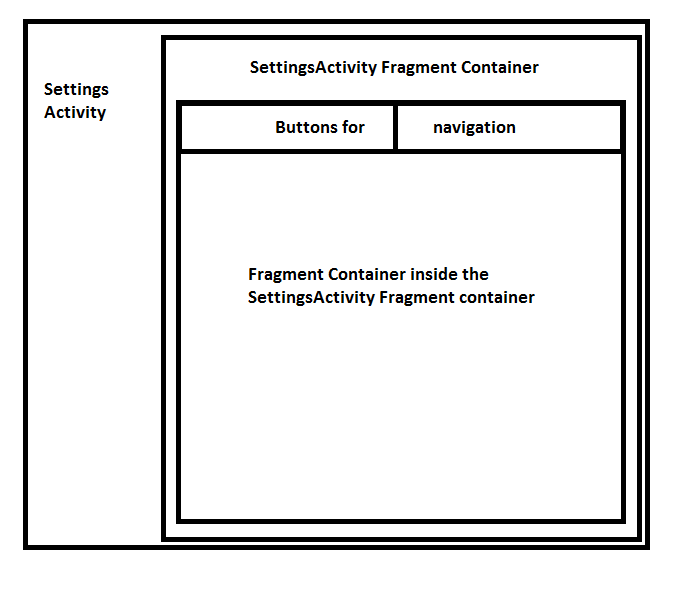
\includegraphics[width=\textwidth, height=3in, keepaspectratio=true] {SettingsActivity.png}
%\caption{The organization of \lstinline!SettingsActivity! when inside the "Apps" pane. Since we need to distinguish between \giraf and Android applications, nested fragment containers are used.}
%\label{fig:settingsappfragments}
%\end{figure}

\subsubsection{AppContainerFragment and the derived classes}

Because the \giraf and Android fragments contain many of the same variables, these inherit all shared information from a superclass, consequently reducing redundancy and clarifying how the two fragments are different.
This superclass is called \lstinline!AppManagementFragment! and the main responsibilities are:

\begin{itemize}
\item Initialize shared variable in \lstinline!onCreate()!
\item Implement shared methods handling when to load applications
\end{itemize}

As a result, the two derived classes get their shared variables initialized by a call to \lstinline!super.onCreate()! and reloading of applications is handled automatically by \lstinline!AppContainerFragment!. \\

However, which type of applications are loaded is different for \lstinline!AndroidFragment! and \lstinline!GirafFragment!.
%As noted in \cref{sec:sprint:designlauncher} and explained in \cref{sect:sprint3:refactoring}, the functions used to load applications into view was moved from \lstinline!HomeActivity! to \lstinline!LauncherUtility!.
This is solved by initializing the shared variable \lstinline!apps! differently in the two derived classes -
\lstinline!GirafFragment! loads \giraf applications into \lstinline!apps!, while \lstinline!AndroidFragment! loads Android applications into it.

Since the automatic load methods mentioned above work on the \lstinline!apps! variable, this solution solves the problem. \\

The other problem present is related to the marking of applications.
%However, one problem has to be directly inside the two derived classes, namely marking the applications as selected and adding them to the users list of selected applications.
This is due to the fact that \giraf applications are saved as the \textit{OasisLib} type \lstinline!Application!, while Android applications are saved as the type \lstinline!ResolveInfo!.

The \giraf applications connected to a user are saved or removed through a call to an \textit{OasisLib} method, while Android applications are saved as a file stored in the native \lstinline!SharedPreferences! of Android.
%Each file name is made, unique to each user, by incorporating the users ID as part of the file name.
More about saving settings in Android can be found in \cref{para:sprint4:managingsettingsandroid} and the code for marking the applications can be seen in \cref{lappendix:markingapps}\\

%This also means that the two fragments must handle the selected applications different, when marking them the first time a fragment is loaded.
%The code is not included, since it is similar to that of \cref{lst:addinggirafapplications} and \cref{lst:addingandroidapplications} - the same checks are carried out, but rather than being for a single application, they are carried out on all installed applications.

These two problems are the main reason we need to derive the two subclasses.\\

Having described all the different types of settings \launcher treats, the next sections explains how to save the settings.

\subsection{Saving Settings}\label{para:sprint4:managingsettingsandroid}
To explain the functionality that saves preferences when a changes has been made, this section describes the features which Android provides for managing preferences on a per application basis. This feature is provided through the \lstinline|SharedPreference| interface.

With this class you can either save the preferences in the context of the application, if they are application specific. It is also possible to define the name of the file in which the preferences are saved or read from. If the preference file does not exist when requested it is created.

We use these features to save preferences for each user. We create a unique file by the user role and id.
This means that a \textit{citizen} profile with the \textit{id 1}, would get the file name \textit{c1}, with the package name of our application as a prefix.

Preferences identified by a key, and they are edited through the Editor class and with a proper method matching the type of the variable which needs to saved, e.g. \lstinline!putBoolean()!.
If the preference exists it is updated if not it is created.

When a preference is to be read it is retrieved by a get method, e.g. \lstinline!getBoolean()!, this method is provided the key for the preference and a default value in case the preference has not yet been set.
